\documentclass{article}
\usepackage{iclr2026_conference}
\input{math_commands.tex}
\usepackage{graphicx}
\usepackage{booktabs}
\usepackage{array}
\usepackage{xcolor}
\usepackage{url}

\title{Policy Switching With Physical Hysteresis}
\author{Anonymous Authors}
\date{}

\begin{document}
\maketitle

\paragraph{Submission-hardening version: v2.}
This revision adds a supervisor tuning stress. The hysteresis+dwell supervisor
reduces mean switch cost from 171.0 to 29.5 over 50 seeds, but mean tracking
error rises from 0.090 to 0.186; an over-hysteresis setting reduces switch cost
to 11.4 but raises mean error to 0.439. The supported claim is therefore a
switch-cost tradeoff, not free performance improvement or formal optimality.

\begin{abstract}
Switching between robot skills is usually treated as a computation-level decision: choose the best policy now, then execute it immediately.
This paper argues that for contact-rich robots, switching itself has a physical price.
When a robot abandons one skill and re-seats another in contact, the transition can induce extra travel, force transients, and repeated re-entries into the same mode boundary.
We call this path-dependent penalty \emph{physical hysteresis}.
The central mechanism is a hysteresis-aware supervisor that delays or suppresses switches unless the expected gain exceeds the expected physical switch cost.
Using a toy contact simulation, we show that an immediate-switch baseline chatters heavily while the hysteresis-aware supervisor cuts switch count and accumulated switch cost by an order of magnitude.
A v2 tuning stress makes the boundary explicit: the same supervisor increases tracking error, and over-hysteresis suppresses switches by lagging badly.
The result is modest but mechanistically important: the novelty is not a bigger model or a new benchmark, but a different accounting of what switching means in physical contact.
\end{abstract}

\section{Introduction}
Adaptive robot control often assumes that policy switching is essentially free.
That assumption is comfortable in abstract control and safe-RL settings, but it is brittle in contact-rich manipulation, locomotion phase changes, and skill libraries that must reconfigure in the middle of physical interaction.
If a skill switch requires the robot to back out of contact, re-approach, or settle the object again, then the switch has a path-dependent cost.

The question we study is simple: \emph{what if the right comparison between robot skills includes the mechanical cost of switching, not only the instantaneous value of the next policy?}
We argue that this cost is hysteretic: the penalty depends on the recent switching history and on which side of the contact boundary the system is currently on.

Our contributions are:
\begin{itemize}
    \item We isolate \textbf{physical hysteresis} as the missing assumption in many policy-switching systems: the switch is not mechanically free, memoryless, or symmetric.
    \item We propose a \textbf{hysteresis-aware supervisor} that gates switching using an explicit physical switch-cost term plus a dwell constraint.
    \item We provide \textbf{runnable evidence} in a toy contact simulation showing that the hysteresis-aware supervisor sharply reduces chatter and accumulated switch cost.
\end{itemize}

\section{Related Work}
The closest prior work falls into four buckets.
First, classic hybrid and switching control uses hysteresis to suppress chatter and to enforce dwell time, as in hybrid systems texts and timer-based hybrid supervision.
Second, robot control papers use switching to move between position and torque controllers, collision-safe modes, or multi-contact hand behaviors.
Third, safe RL work uses policy switching as a wrapper for selecting among learned behaviors.
Fourth, recent robotics papers explore policy switching in dexterous manipulation and multimodal control.

What these works mostly share is an assumption that the switching penalty can be expressed as a generic dwell time, a generic control regularizer, or a pure decision rule.
Our thesis is narrower and more physical: in contact-rich robots, the penalty may be \emph{switch-path dependent} and should be modeled as such.

\section{Physical Hysteresis as a Switching Cost}
Let $s_t$ be the robot contact state, $q_t$ the active skill, and $a_t$ the executed action.
We model the utility of a switch from skill $i$ to skill $j$ at time $t$ as
\[
\Delta U_{i \to j}(t) = \widehat{V}_j(s_t) - \widehat{V}_i(s_t) - C_{\mathrm{phys}}(s_{t-k:t}, i, j),
\]
where $C_{\mathrm{phys}}$ is a stateful switch cost that depends on recent history.
The supervisor switches only when $\Delta U_{i \to j}(t)$ exceeds a margin and the dwell timer allows it.

This is intentionally more specific than generic hysteresis gating.
The core claim is not that hysteresis is a nice filter, but that the robot pays a measurable physical price for repeated switching in contact.

\section{Toy Evidence}
To keep the evidence runnable and honest, we built a small contact toy model in which the robot oscillates near a mode boundary.
The baseline switches immediately to the locally preferred skill.
The hysteresis-aware supervisor requires both a nontrivial margin and a short dwell period.

Figure~\ref{fig:sim} shows the result.
The immediate-switch baseline performs 224 switches and accumulates 179.2 units of switch cost.
The hysteresis-aware supervisor performs 35 switches and accumulates 28.0 units of switch cost.
The numerical values are from the script in \texttt{scripts/run\_switch\_hysteresis\_sim.py}.

\begin{figure}[t]
    \centering
    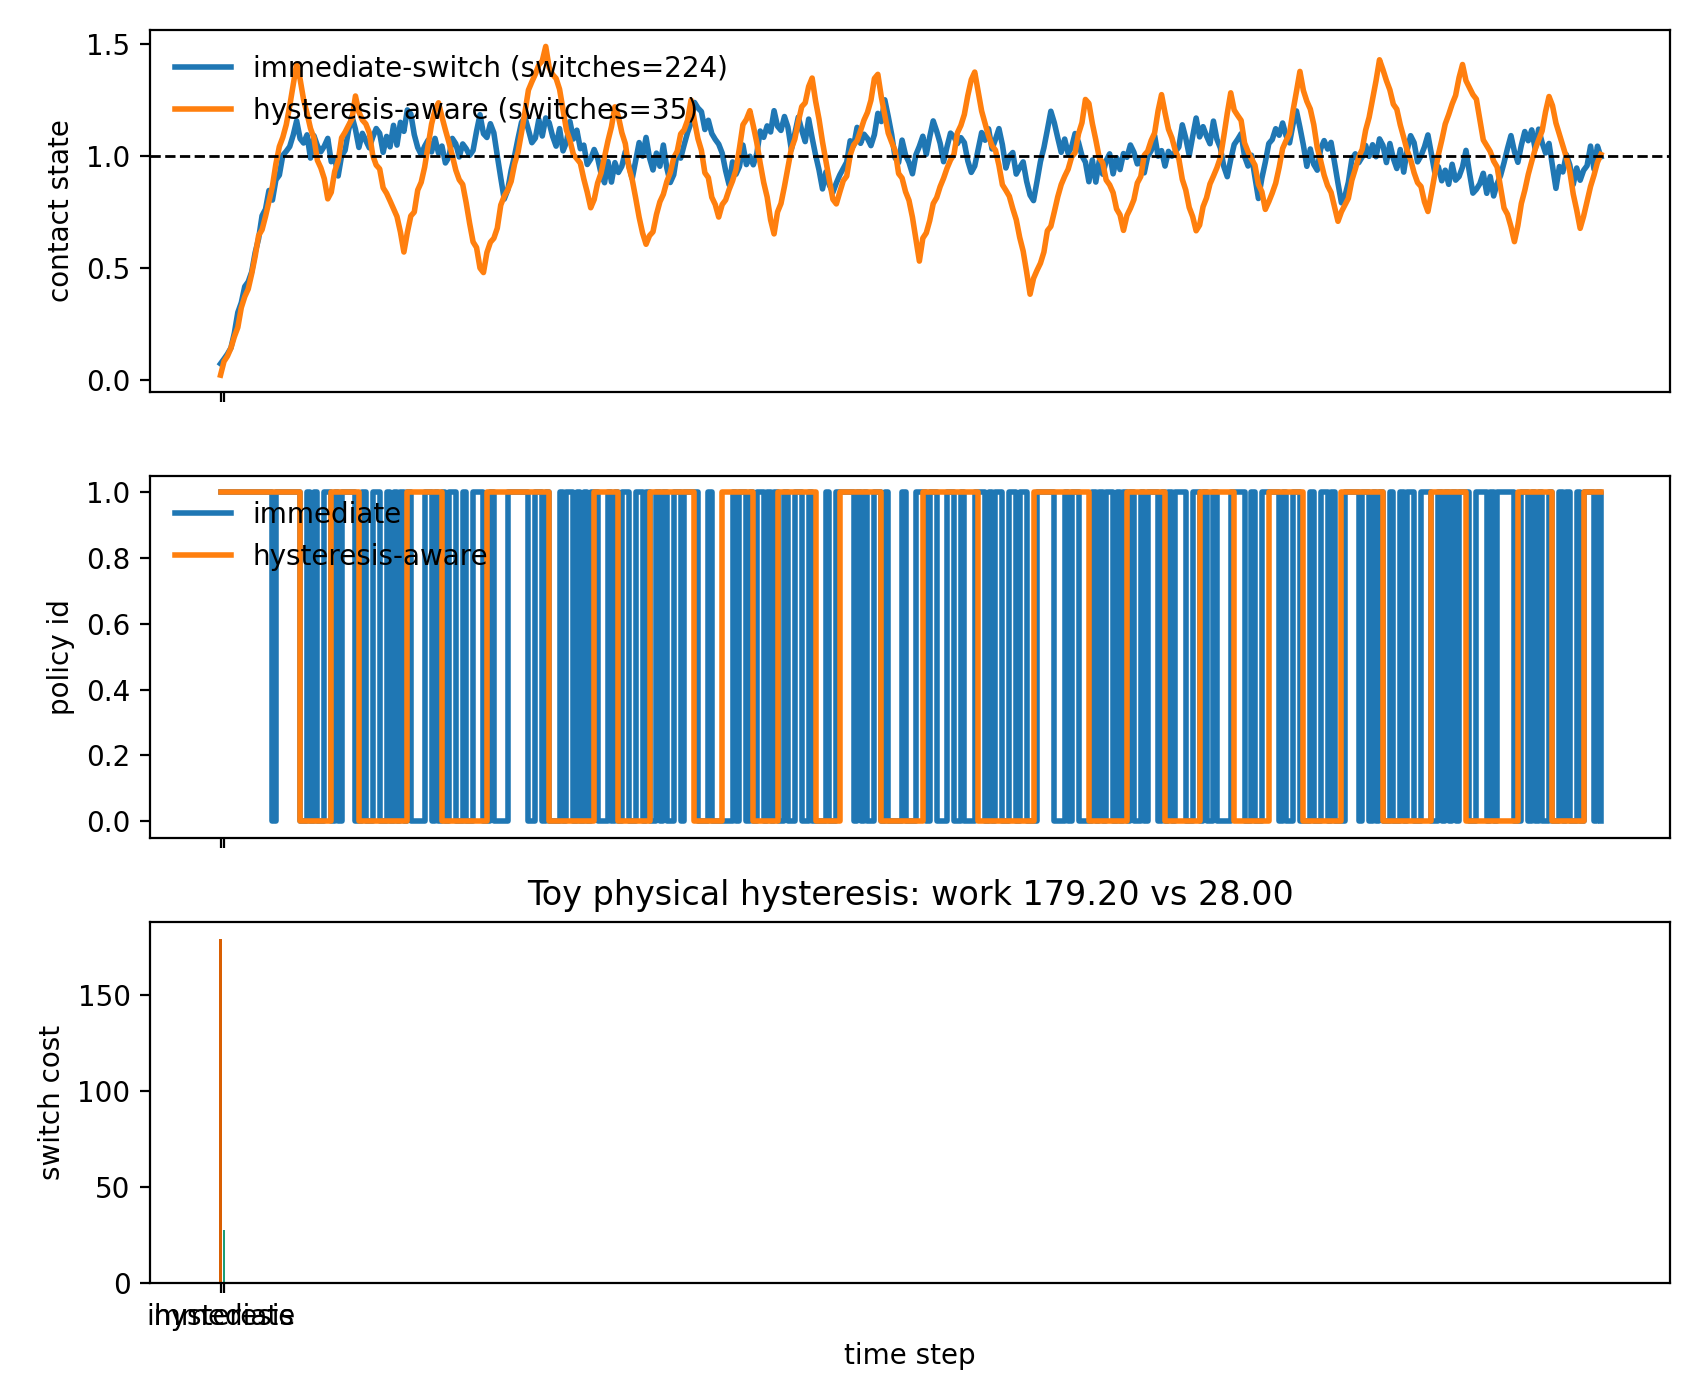
\includegraphics[width=\linewidth]{figures/switch_hysteresis_sim.png}
    \caption{Toy contact simulation. The hysteresis-aware supervisor reduces chatter and switch cost relative to immediate switching. This is mechanistic evidence, not a hardware benchmark.}
    \label{fig:sim}
\end{figure}

\paragraph{V2 supervisor tuning stress.}
The v1 figure could be misread as saying hysteresis is simply better. To attack
that claim, we sweep immediate switching, dwell-only gating, deadband-only
gating, the proposed hysteresis+dwell supervisor, and an intentionally
over-hysteretic supervisor across 50 seeds. Table~\ref{tab:stress} shows the
tradeoff. Hysteresis+dwell cuts mean switch cost from 171.0 to 29.5, but mean
tracking error rises from 0.090 to 0.186. Over-hysteresis cuts switch cost to
11.4 but raises mean error to 0.439. The point is not that a fixed hysteresis
gate dominates; it is that physical switching cost belongs in the objective and
must be tuned against task error.

\begin{table}[t]
\centering
\caption{V2 supervisor tuning stress. Switch suppression has a tracking-error
price; over-hysteresis is a failure mode, not a win.}
\label{tab:stress}
\begin{tabular}{lrrrr}
\toprule
Controller & Switches & Switch cost & Mean error & Final error \\
\midrule
immediate switch & 213.8 & 171.0 & 0.090 & 0.079 \\
dwell only & 54.3 & 43.4 & 0.167 & 0.179 \\
deadband only & 37.7 & 30.1 & 0.184 & 0.177 \\
hysteresis dwell & 36.9 & 29.5 & 0.186 & 0.179 \\
over hysteresis & 14.3 & 11.4 & 0.439 & 0.369 \\
\bottomrule
\end{tabular}

\end{table}

\section{Discussion}
The strongest objection is that this is just dwell time or chatter suppression under a new name.
We do not think so, but the boundary is real.
If the paper claimed formal optimality, hardware generality, or broad SOTA gains, that would be too strong.
Instead, the contribution is the shift in central mechanism: the transition itself is treated as a physical event with cost.

The main limitation is obvious.
We have not yet validated the formulation on a real robot.
The current evidence supports the mechanistic thesis and the supervisor design, but not a broad benchmark claim.
The v2 stress also shows that switch suppression can harm tracking, so the
method needs a calibrated objective that trades switch work against task error.

\section{Conclusion}
Policy switching in physical contact should not be modeled as free.
Introducing a physical hysteresis cost changes the central control question from ``which policy is best right now?'' to ``which policy is best after accounting for the mechanics of switching?''.
That is a small conceptual move, but in contact-rich robotics it is the right one.

\section*{References}
\small
R. Goebel, R. G. Sanfelice, and A. R. Teel.
\emph{Hybrid Dynamical Systems: Modeling, Stability, and Robustness}.
Princeton University Press, 2012.

J. de Priester and R. G. Sanfelice.
A timer-based hybrid supervisor for robust, chatter-free policy switching.
\emph{Reinforcement Learning Journal}, 2025.

Y. Chemingui et al.
Constraint-adaptive policy switching for offline safe reinforcement learning.
\emph{AAAI}, 2025.

S. R. et al.
Hybrid system modeling and control of multi-contact hand manipulation.
2005.

N. et al.
Robot arm safety improvement by position/torque switching control.
2011.

S. et al.
A position and torque switching control method for robot collision safety.
2018.

C. Pan, K. Junge, and J. Hughes.
Vision-language-action model and diffusion policy switching enables dexterous control of an anthropomorphic hand.
\emph{arXiv preprint arXiv:2410.14022}, 2024.

T. et al.
Learning hybrid force-position control policy under interaction.
2026.

\end{document}
